\documentclass{kuisthesis}
\usepackage{listings}
\usepackage[dvipsnames]{xcolor}
\usepackage{amsmath,amssymb}
\usepackage{comment}
\usepackage[dvipdfmx]{graphicx}

\definecolor{base}{gray}{0}
\definecolor{comment}{named}{Green}
\definecolor{string}{named}{Red}
\definecolor{keyword1}{named}{Cyan}
\definecolor{keyword2}{named}{Magenta}
\definecolor{keyword3}{named}{YellowOrange}
\definecolor{keyword4}{named}{Violet}


\lstdefinelanguage{michelson}{
  morekeywords = [1]{
    int, nat, bool, pair, operation, list, unit, mutez
  },
  morekeywords = [2]{
    parameter, storage, code
  },
  morekeywords = [3] {
    CAR, DUP, DIP, CDR, ADD, NIL, PAIR, GT, LOOP, PUSH, IF, ITER, AMOUNT, COMPARE, EQ, IF, SOURCE, CONTRACT, IF_NONE, FAILWITH, UNIT, TRANSFER_TOKENS, CONS
  },
  morecomment = [l]{//},
  morecomment = [s]{/*}{*/},
  morestring = [b]{"},
  morestring = [b]{'},
  alsodigit = {-},
  sensitive = true
}

\renewcommand{\lstlistingname}{Code}
\lstset{
  basicstyle={\ttfamily\color{base}\small},%コードの基本書式
  keywordstyle=[1]{\color{keyword1}},%キーワード1のスタイル
  keywordstyle=[2]{\color{keyword2}},%キーワード2のスタイル
  keywordstyle=[3]{\color{keyword3}},%キーワード3のスタイル
  keywordstyle=[4]{\color{keyword4}},%キーワード4のスタイル
  commentstyle={\gtfamily\color{comment}},%コメントのスタイル
  stringstyle={\gtfamily\color{string}},%文字列のスタイル
  numbers=left,%行番号は左
  stepnumber=1,%一行ずつ行番号をふる
  numberstyle={\sffamily\scriptsize},%行番号の書式
  xleftmargin=0zw, %左余白
  xrightmargin=0zw,%右余白
  tabsize=4,%タブの空白数
  frame=single,%フレームの書式
  frameround=tttt,%角を丸めるかどうか tで丸める
  breaklines=true,%長くなったら途中で改行
  captionpos=b,%タイトルの位置
  breakindent=10pt,%改行されたときの送り幅
  showstringspaces=false,%文字列中の半角スペースを表示させない
  lineskip=-1pt%通常の文章より行送りを狭くする
}

\jtitle[スマートコントラクトのガス消費量のResource Aware MLを\\用いた静的解析]
  {スマートコントラクトのガス消費量の\\Resource Aware MLを用いた静的解析}
\etitle{Static Analysis for Gas Consumption of Smart Contracts Using Resource Aware ML}
\jauthor{小野 雄登}
\eauthor{Yuto Ono}
\supervisor{末永 幸平 准教授}
\date{2021年2月2日}

\begin{document}
\maketitle

\begin{jabstract}
2008年にビットコインが開発されて以来,
現在に至るまでにブロックチェーンを技術基盤とする様々な仮想通貨が開発されている.
\emph{スマートコントラクト}は,仮想通貨の取引における契約の締結や履行を自動化する仕組みであり,
ブロックチェーン上で動作するプログラムとして実装される.

スマートコントラクトには\emph{ガス}の概念が存在する.
ガスはコントラクトの実行のために利用する計算資源にかかる手数料を表している.
コントラクトが実行される際に,コントラクトの各命令の実行毎に命令の計算コストに応じた量のガスが消費される.
消費量の合計が許容ガス消費量を超えると,プログラムの実行が直ちに停止され,プログラムの実行による効果がロールバックされる.
コントラクトを実行しようとする際は,あらかじめ一定量のガスに相当する通貨を支払う必要があるが,これは実行が取り消されても返金されない.
このような実行コストの無駄をを抑えるために,ガスの消費量を静的に解析する手法が求められている.

プログラムの実行コストを解析する手段の一つとして,\emph{Resource Aware ML\ (RAML)}\ がある.
RAMLは,ポテンシャルベースの償却解析と呼ばれる,データ構造の状態に応じてコストが変わる一連の操作のコストを解析する手法をもとに設計された,
OCamlで用いられる文法を備えた関数型プログラミング言語である.
RAMLは入力として与えられたプログラムのリソース消費量の上界を,
指定されたメトリックに従って自動的に,かつ静的に解析して,その結果を出力するツールとして用いることができる.

本研究では,RAMLを用いて,仮想通貨Tezosのスマートコントラクトのガス消費量を静的に解析する手法を提案する.
Tezosのスマートコントラクトは,スタックベースのプログラミング言語Michelsonで記述される.
このプログラムをRAMLで解析するために,Michelsonにおいて実装されている各命令の挙動を模倣するライブラリをRAMLで実装する.
このライブラリを用いて,Michelsonプログラムの挙動を模倣するRAMLプログラムを作成することができる.
また,そのプログラムをRAMLで解析することで,プログラムのガス消費量を見積もることができる.

Michelsonの命令は受け取ったスタックを書き換える.
この挙動をRAMLで再現するために,スタックの要素をヴァリアント型{\tt t}として定義し,スタックを型{\tt t}のリストとして扱い,
命令を({\tt t list $\rightarrow$ t list})型をもつ関数として定義する.
Michelsonのコントラクトは,初期スタックに積まれる値の型宣言と,
初期スタックに対して順に適用される一連の命令によって構成されている.
この動作を模倣するプログラムを,本ライブラリを用いて,
初期スタックを表すリストに対して命令を順に関数適用するプログラムとして実装することができる.

Tezosのコントラクトの実行に伴うガスの消費量のうち,本研究では特に
プログラムの解釈実行を行う際に発生する\emph{interpreter cost}を見積もることを目的とする.
各命令のガス消費量はRAMLのtickメトリックを用いて表現する.
tickメトリックは,リソースの消費量や発生するタイミングをユーザーが定義するためのメトリックで,
RAMLに備えられている関数を呼び出すことでその関数のリソース消費量を定義することができる.
本ライブラリの各命令について,その命令のinterpreter costに相当する値の関数を呼び出すよう定義し,
tickメトリックを用いて,コントラクトを模倣するプログラムの解析を行い,コントラクトのinterpreter costを見積もる.

いくつかのMichelsonコントラクトを模倣するRAMLプログラムを作成し,それに対して解析を行いガス消費量の見積もりを行った.
その結果,基本的なスタック操作や条件分岐の命令のみで構成されているコントラクトについては解析が成功し,
interpreter costを正しく見積もることができた.
一方で,リストに対する再帰を行う命令を含むコントラクトでは解析が行えなかった.
また,ガス消費量がスタック中の値に依存するような命令を含むコントラクトについては,
正しくinterpreter costの見積もりを行うことは難しかった.

本研究において実装しなかった命令や,解析が正しく行えなかった命令を扱えるようにライブラリを拡張することは,今後の課題である.
また,コントラクトの実行において発生するその他のコストの見積もり,
ひいてはコントラクトの実行コスト全体の見積もりについても検討していく.


\end{jabstract}

\begin{eabstract}
Since the development of BitCoin in 2008, a variety of cryptocurrencies based on blockchain technology have been developed. 
Many cryptocurrencies support \emph{smart contracts}, which are programs executed on a blockchain.
A smart contract is used to execute a transaction involving cryptocurrencies automatically.

There is a concept of \emph{gas consumption} in smart contracts. 
Gas is the fee for the computational resources used to execute a contract.
When a contract is executed,  the execution of each instruction consumes gas corresponding to its computational cost.
If the total consumption exceeds the prespecified amount, the execution of the program is aborted immediately and the effect of the program execution is rolled back.
One who would like to execute a contract is required to pay cryptocurrency equal to the expected amount of the gas consumption in advance, which is not refunded even if the execution is aborted due to an out of gas error.
A method to statically analyze the gas consumption is therefore required to avoid such trouble.

\emph{Resource Aware ML\ (RAML)\ } is one of the methods to analyze the execution cost of a program.
RAML is a functional programming language equipped with the OCaml syntax.
Using the potential-based amortized analysis, which is an analysis of the costs of a sequence of operations whose costs vary depending on the state of the data structure,
RAML automatically and statically analyzes the resource consumption bounds for a given program for a specified metric.

This study proposes a method to statically analyze the gas consumption of a smart contract of cryptocurrency Tezos using RAML.
A Tezos smart contract is written in a stack-based programming language Michelson.
To this end, we implemented a library in RAML each function of which imitates the behavior of each Michelson instruction.
Using this library, we can write a RAML program that imitates the behavior of a Michelson program.
Then, we can estimate the gas consumption of the program by analyzing it with RAML.

Since a Michelson instruction rewrites the stack, we implemented a RAML function that imitates each Michelson instruction as one with {\tt (t list $\rightarrow $ t list)}, where {\tt t} is the variant type that expresses stack elements and {\tt t list} is the type that expresses a stack.
Then we can implement a RAML program that imitates the behavior of a Michelson program as one that applies the functions in our library to the initial stack.

Although the gas consumption of execution of a Tezos contract consists of several types of costs, we aim at estimating the \emph{interpreter cost}, which is for executing a Michelson program.
For this purpose, we use the \emph{tick metric} of RAML, which is used for defining the quantity of custom resource consumption.
We can define the resource consumption of a function by calling a primitive function provided by RAML. 
We implemented the library so that each function calls the function that expresses its interpreter cost.
By encoding a contract with our library as a RAML program, we can estimate the interpreter cost of the contract by analyzing the RAML program with the tick metric.

We encoded several Michelson contracts to RAML programs using our library and analyzed them to estimate the gas consumption.
The analysis was successful for the contracts that consisted only of instructions of basic stack operations and conditional branches; the estimation was correct for these contracts.
However, the analysis was not successful for contracts that contain instructions for recursion on lists.
RAML could not analyze the interpreter cost of contracts that contain instructions whose gas consumption depends on the contents of the stack.

Extension of the library to cover more Michelson instructions and to handle recursion on lists are left as future work.
We also plan to study other types of costs than the interpreter cost and estimate them.


\end{eabstract}

\tableofcontents

\section{序論}\label{sec-intro}
2008年にビットコインが開発されて以来\cite{bitcoin},
現在に至るまでにブロックチェーンを技術基盤とする様々な仮想通貨が開発され,分散ネットワーク上での取引が活発化している.
取引の記録をブロックとしてネットワーク上に記憶するという性質上,ブロックチェーンはデータ改竄に対する優れた耐性を持ち,
仮想通貨の取引を支えるコア技術となっている.
ブロックチェーン上で用いられる技術として\emph{スマートコントラクト}がある.
スマートコントラクトは,仮想通貨の取引における契約の締結や履行を自動化する仕組みであり,
ブロックチェーン上で動作するプログラムとして実装される.

スマートコントラクトには\emph{ガス}の概念が存在する\cite{tezos}.
ガスはコントラクトの実行のために利用する計算資源にかかる手数料を表している.
コントラクトが実行される際に,コントラクトの各命令の実行毎に命令の計算コストに応じた量のガスが消費される.
ガスの消費量の合計が計算されると,それが通貨に変換され,ブロックの生成者であるマイナーに対して払われる手数料となる.
コントラクトの実行者は,実行前にガス消費量の上限となるガス許容量を設定し,
消費量の合計が許容量を超えると,プログラムの実行が直ちに停止され,プログラムの実行による効果がロールバックされる.
また,コントラクトを実行しようとする際は,あらかじめ一定量のガスに相当する通貨を支払う必要があるが,これは実行が取り消されても返金されないため,
実行コストが無駄にかかってしまうことになる.
このような無駄なコストを削減し,コントラクトの実行コストを抑えるために,
コントラクトの実行者は実際のガス消費量より大きいが,大幅には上回らないガス許容量を設定することが望ましい.
そのために,ガスの消費量を静的に解析する手法が求められている.

本研究では,仮想通貨Tezosのスマートコントラクトのガス消費量を静的に解析する手法を提案する.
Tezosはスマートコントラクトを用いたブロックチェーンを技術基盤とする仮想通貨の1つで,
そのスマートコントラクトはスタックベースのプログラミング言語Michelsonで記述される.

解析を行う手法として,本研究では\emph{Resource Aware ML\ (RAML)}\ \cite{raml}を用いる.
RAMLは,ポテンシャルベースの償却解析と呼ばれる,データ構造の状態に応じてコストが変わる一連の操作のコストを解析する手法をもとに設計された\cite{amortized},
OCamlで用いられる文法を備えた関数型プログラミング言語である.
RAMLは入力として与えられたプログラムのリソース消費量の上界を,
指定されたメトリックに従って自動的に,かつ静的に解析して,その結果を出力するツールとして用いることができる.

MichelsonのプログラムをRAMLで解析するために,Michelsonの各命令の挙動を模倣するライブラリをRAMLで実装する.
このライブラリを用いて,Michelsonプログラムを模倣するRAMLプログラムを作成する.
そのRAMLプログラムを,RAMLに備えられているメトリックの一つであるtickメトリックを用いて,
コントラクトのガス消費量のうち,プログラムの解釈実行を行う際に発生するinterpreter costの見積もりを行う.
以上のような手法で,いくつかのコントラクトの解析を行った結果,
単純な命令のみで構成されているコントラクトのinterpreter costを正しく見積もることができた.
一方,interpreter costが複雑な計算によって算出されるような命令を含むコントラクトについては見積もりが難しく,
今後の課題である.

本報告書は以下のように構成されている.第2章では,本研究の背景知識として,TezosとMichelson,
スマートコントラクトにおけるガス消費の仕組み,そして解析に用いるRAMLについてそれぞれ説明する.
第3章では, Michelsonプログラムを模倣するRAMLプログラムの実装について説明する.
第4章では,コントラクトのガス消費量の解析についていくつかの例を挙げ,結果と考察を述べる.
第5章では,本研究の関連研究について論ずる.
最後に第6章で本研究についての結論を述べる.


\section{背景知識}\label{sec-preliminary}
本節では,本研究に関連する背景知識について述べる.第2.1節ではTezosとMichelsonについて,
第2.2節ではスマートコントラクトにおけるガス消費の仕組みについて,
第2.3節ではRAMLについてそれぞれ述べる.

\subsection{TezosとMichelson}\label{subsec-pre-tezos}
Tezosはスマートコントラクトを用いたブロックチェーンを技術基盤とする仮想通貨の1つである.
BitcoinやEthereumといった仮想通貨が先立って流通されるようになった中,
Tezosはそれらのブロックチェーンの弱点を解消することを目的として開発された\cite{tezos}.
Tezosの特徴として\emph{Proof-of-Stake}\ (PoS)\ と呼ばれるコンセンサスアルゴリズムを採用していることが挙げられる.
従来のブロックチェーンで採用されている\emph{Proof-of-Work}\ (PoW)\ が,
コンピュータの計算能力が高いユーザーに対してブロック生成の権利を与えているのに対して,
PoSでは通貨の保有量が多いユーザーに対してブロック生成の権利が与えられる.
Tezosの採用しているPoSは\emph{Liquid Proof-of-Stake}\ (LPoS)\ といい,
ブロック生成の権利を他のユーザーに委任することができる.
これにより,多くのユーザーがブロック生成に参加することができ,
プロトコルの分散性を高めるという目的に寄与している.

 Michelsonは,Tezosのスマートコントラクトを記述するために用いられるプログラミング言語である.
この言語はスタックベースで,高レベルのデータ型とプリミティブ,および厳密な静的型チェックを備えている\cite{michelson}.


\begin{figure}[ht]
  \begin{center}
    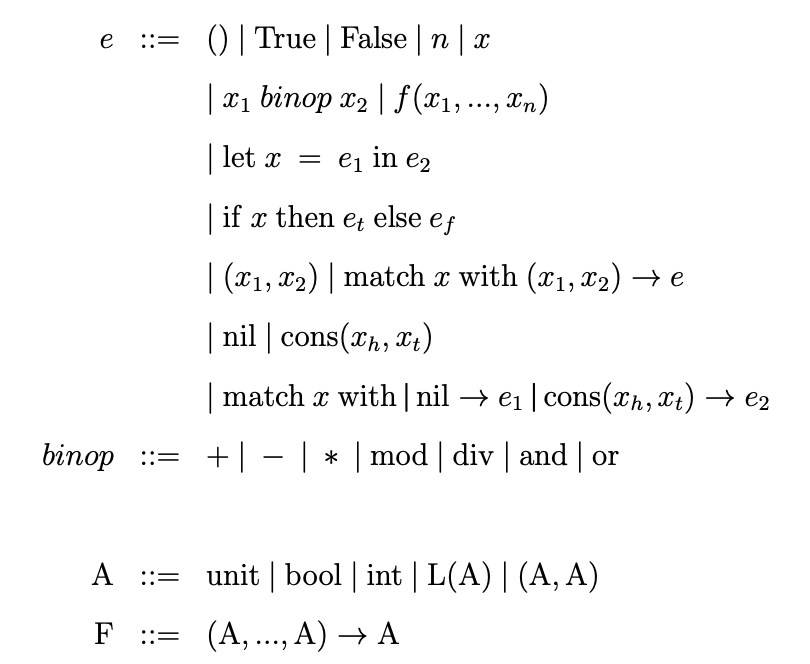
\includegraphics[scale=0.75]{image1.png}
    \caption{Michelsonの文法}
    \label{image1}
  \end{center}
\end{figure}


\begin{comment}
\begin{eqnarray*}
  T &::=& {\tt int\ |\ nat\ |\ mutez\ |\ bool\ |\ address\ |\ unit}\ |\\
  && {\tt option}\ T\ |\ {\tt list}\ T\ |\ {\tt operation\ |\ contract}\ T\ |\ {\tt pair}\ T\ T\ |\ {\tt or}\ T\ T \\
  V &::=&\ i\ |\ {\tt True\ |\ False}\ |\ a\ |\ {\tt Unit}\ |\ (V_1, V_2)\ |\ {\tt Left}\ V\ |\ {\tt Right}\ V\ |\\
  && {\tt Some}\ V\ |\ {\tt None\ |\ []}\ |\ V_1 :: V_2\ |\ IS\\
  n &::=& [0-9]+ \\
  i &::=& n\ |\ -n \\
  IS &::=& \{I_1;\ ...\ ;I_n\} \\
  I &::=& {\tt FAILWITH\ |\ IF}\ IS_1\ IS_2\ |\ {\tt LOOP}\ IS\ |\ {\tt DIP}\ IS\ | \\
  && {\tt DROP\ |\ DUP\ |\ SWAP\ |\ PUSH}\ T\ V\ |\ {\tt UNIT}\ |\\
  && {\tt EQ\ |\ NEQ\ |\ LT\ |\ GT\ |\ LE\ |\ GE\ |\ OR\ |\ AND\ |\ XOR\ |\ NOT}\ | \\
  && {\tt NEG\ |\ ABS\ |\ ISNAT\ |\ INT\ |\ ADD\ |\ SUB\ |\ MUL\ |\ EDIV}\ |\\
  && {\tt COMPARE\ |\ PAIR\ |\ CAR\ |\ CDR\ |\ SOME\ |\ NONE}\ T\ |\\
  && {\tt IF\_NONE}\ IS_1\ IS_2\ |\ {\tt LEFT}\ T\ |\ {\tt RIGHT}\ T\ |\ {\tt IF\_LEFT}\ IS_1\ IS_2\ | \\
  && {\tt NIL}\ T\ |\ {\tt CONS\ |\ IF\_CONS}\ IS_1\ IS_2\ |\ {\tt SIZE\ |\ MAP}\ IS\ |\ {\tt ITER}\ IS\ | \\
  && {\tt CONTRACT}\ T\ |\ {\tt TRANSFER\_TOKENS\ |\ AMOUNT\ |\ SOURCE} \\
  S &::=& {\tt E}\ |\ V : S
\end{eqnarray*}
\end{comment}

Michelsonの文法のうち,本研究でRAMLで実装する部分の文法を図\ref{image1}に示す.
$T$はスタックの要素の型を表す.$T$は整数値の型{\tt int},自然整数の型{\tt nat},Tezosの通貨量の型{\tt mutez},
Booleanの型{\tt bool},アドレスを表す型{\tt address},Unit値の型{\tt unit},オプション値の型{\tt option},
命令を表す型{\tt operation},コントラクトを表す型{\tt contract},ペアの型{\tt pair},ユニオンの型{\tt or}がある.
$V$はスタックの要素の値を表し,整数値の$i$,Booleanの{\tt True,False},アドレスの$a$,
Unit値の{\tt Unit},ペアの($V_1,V_2$),ユニオンの{\tt Left} $V$,{\tt Right} $V$,
オプション値の{\tt Some} $V$,{\tt None},空リストの[\ ],リストの結合を表す$V_1 :: V_2$,
命令列$IS$がある.$n$は自然数,$i$は整数である.
$IS$は命令列で,命令$I$のシーケンスである.
命令$I$は,プログラムを中止する命令({\tt FAILWITH}),構造のコントロールに関する命令({\tt IF,LOOP,DIP}),
スタックの操作に関する命令({\tt DROP,DUP,SWAP,PUSH,UNIT}),
スタックのトップ要素の比較に関する命令({\tt EQ,NEQ,LT,GT,LE,GE}),
Booleanに関する操作の命令({\tt OR,AND,XOR,NOT}),
整数値に関する命令({\tt NEG,ABS,ISNAT,INT,ADD,SUB,MUL,EDIV}),
スタックの上から2つの要素の比較命令({\tt COMPARE}),ペアに関する命令({\tt PAIR, CAR,CDR}),
オプション値に関する命令({\tt SOME,NONE,IF\_NONE}),ユニオンに関する命令({\tt LEFT,RIGHT,IF\_LEFT}),
リストに関する命令({\tt CONS,NIL,IF\_CONS,MAP,SIZE,ITER}),
コントラクトに関する命令(C{\tt ONTRACT,TRANSFER\_TOKENS,AMOUNT,SOURCE})がある.
$S$はスタックを表す.空のスタックを{\tt E}で表し,スタックに積まれた要素は\ :\ で区切る.
空のスタックを表す{\tt E}は,要素の積まれたスタックを表すときは省略する.
例えば,$V_1 : V_2$は$V_1 : V_2 : {\tt E}$を省略した形である.




Michelsonのプログラムは,プログラムに対して与えられるパラメータと,ブロックチェーン上に保存されているストレージのペアを受け取り,
このプログラムの終了後に実行される操作のリストと,
プログラムの実行中に更新されブロックチェーン上に保存されるストレージのペアを返す純粋な関数である.
プログラムの本体は,順番に実行される一連の命令である.
各命令は,スタックを入力として受け取り,そのスタックの内容を書き換えて出力する.
プログラムの初期スタックは,引数として与えられたパラメータとストレージのペアが一番上に積まれた状態のもので,
その初期スタックに対して順番に命令が適用され,
最後に操作のリストとストレージのペアが一番上に積まれた状態のスタックが残り,それが出力される.

Michelsonプログラムの例として,簡単な演算を行うプログラムであるexample1のコードをCode \ref{ex1tz}に示す.
これは,整数のペアをパラメータとして受け取り,2つの整数の和をストレージに書き込むプログラムである.
なお,各命令後のスタックの状態を/*,*/で囲われたコメントで示している.
\begin{lstlisting} [language=michelson, caption=example1.tz, label=ex1tz]
parameter (pair int int); 
storage int;
code  /* ((para1, para2), st) */
  { CAR ;   /* (para1, para2) */
    DUP ;   /* (para1, para2) : (para1, para2) */
    CAR ;   /* para1 : (para1, para2) */
    DIP { CDR } ;   /* para1 : para2 */
    ADD ;   /* st' */
    NIL operation ;   /* [] : st' */
    PAIR }   /* ([], st') */
\end{lstlisting}

以下,プログラムの内容を説明する.

Michelsonプログラムのコードは,プログラムに対して与えられる引数である{\tt parameter}と,
ブロックチェーン上に保存されているストレージの値である{\tt storage}の型宣言から始まる.
1行目は{\tt parameter}の型が({\tt pair int int})であること,2行目は{\tt storage}の型が{\tt int}であることを宣言している.
3行目以降はプログラムの本体である{\tt code}である.{\tt code}には一連の命令が記述されていて,
この命令が初期スタックに対して順に実行されていく.以下,{\tt code}の内容について行番号ごとに説明する.

\begin{itemize}
  \item {\tt プログラム開始時のスタックは,parameterとstorageの値のペアが空のスタックに積まれた状態で始まる.
  parameterの値を(para1, para2),storageの値をstと表すとすると,初期スタックは((para1, para2), st)である}.
  \item 4行目の{\tt CAR}は,スタックのトップの要素がペアだった場合,その要素を取り出して,
  ペアの第1要素をスタックに積む命令である.4行目時点でのスタックは{\tt (para1, para2)}である.
  \item 5行目の{\tt DUP}は,スタックのトップの要素を複製してスタックに積む命令である.
  5行目時点でのスタックは{\tt (para1, para2)} : {\tt (para1, para2)}である.
  \item 6行目は4行目と同じく{\tt CAR}を実行する.6行目時点でのスタックは{\tt para1} : {\tt (para1, para2)}である.
  \item 7行目の{\tt DIPは引数として命令列bodyを受け取る命令で,スタックのトップの要素を保持した状態で,
  その要素を取り出した状態のスタックに対してbodyを実行する命令である.
  つまり,スタックのトップのpara1を保持した状態で,スタック(para1, para2)に対してCDRを実行する.
  CDR}は,スタックのトップの要素がペアの場合,その要素を取り出して,ペアの第2要素をスタックに積む命令である.
  よって,7行目時点でのスタックは{\tt para1} : {\tt para2}である.
  \item 8行目の{\tt ADD}は,スタックのトップの要素{\tt x}と2番目の要素{\tt y}の型が,それら2つの演算が定義されているような型である場合,
  {\tt xとyを取り出し,x + yの値をスタックに積む命令である.例えば,xとyがともにint型ならば,x + yはint型である.
  para1 + para2の値をst'}と表すとすると,8行目時点でのスタックは{\tt st'}である.
  \item 9行目の{\tt NILは引数として型aを受け取る命令で,リストの型がaであるような空のリスト[]}をスタックに積む命令である.
  9行目時点でのスタックは{\tt []} : {\tt st'}である.
  \item 10行目の{\tt PAIR}はスタックのトップの要素と2番目の要素を取り出し,それらのペアをスタックに積む命令である.
  この命令後,スタックは{\tt ([], st')}となり,プログラムが終了する.
\end{itemize}

プログラムの終了時のスタックは,このプログラム終了後に続いて行われる操作のリスト{\tt operation listと,
実行中に更新されブロックチェーンに保存されるストレージの値storage'のペアのみが積まれている状態でなければならない.
このとき,プログラム実行前のストレージの値storageと,プログラム実行後のストレージの値storage'の型が一致している必要がある.}

Michelsonには静的型検査が備えられている.それぞれの命令には,
命令の実行前と実行後のスタックの状態を型で表した型付け規則が存在する.
例えば,{\tt PAIR}についての型付け規則は以下のように表される.
\begin{displaymath}
  {\tt a' : b'} : S' \rightarrow {\tt pair\ a'\ b'} : S'
\end{displaymath}
これは,実行前のスタックのトップの要素の型が{\tt a',2番目の要素の型がb'のとき,
実行後のスタックのトップの要素がpair a' b'となることを示している.
また,ADDについての型付け規則は以下のように表される.}
\begin{displaymath}
  {\tt int : int} : S' \rightarrow {\tt int} : S'
\end{displaymath}
これは,実行前のスタックのトップの要素と2番目の要素がともに{\tt intである必要があり,
その場合,実行後のスタックのトップの要素がint}となることを示している.

命令を実行する前にスタックの状態が型付け規則に則った形でない場合,命令は失敗する.
これを防ぐために,プログラム実行前に静的な型検査が行われる.

\subsection{コントラクトのガス消費の仕組み}\label{subsec-pre-gas}
スマートコントラクトにおけるガスは,コントラクトを実行させる上で必要となる手数料を表している.
スマートコントラクトを実行する際,ブロックの生成者であるマイナーがそのコントラクトの検証を行い,
その対価としてコントラクトの実行者がマイナーに対して手数料を支払う必要がある.
この手数料を計算する際にガスという概念が用いられており,計算されたガスの消費量はそのブロックチェーンで用いられる通貨に変換される.


ガス消費量の計算については,コントラクトが実行される際に,
コントラクトの各命令の実行毎に命令の計算コストに応じた量のガスが消費される.
ガスの消費量の合計が計算されると,それが通貨に変換され,マイナーに対して支払う手数料となる.
また,これとは別にあらかじめ一定量のガスに相当する通貨をマイナーに対して支払う必要がある.
コントラクトの実行者は実行時にガスの上限値を設定し,ガスの消費量の合計がその上限値を超えると,
プログラムの実行が直ちに停止され,プログラムの実行による変更が取り消される.
このとき,実行が取り消された場合でも,あらかじめ支払った通貨は返金されないので,
無駄なコストとなってしまう.

以降は,Tezosにおけるガス消費量の計算について述べる.
Tezosにおいて,トップレベルのコードや関数値,型などの値は全てバイト列として保存され,送信される.
コントラクトの実行において発生するガスの消費量は,以下の8つのコストに分けられていて,それぞれ計算方法や発生するタイミングが異なる.

\begin{enumerate}
  \item データベースにアクセスして,必要とする値が存在するかどうか確認し,その値を読み込む.
  このとき,reading costと呼ばれるコストが発生する.
  \item バイト列は,型なしの中間表現であるMicheline表現へと逆シリアル化される.
  このとき,deserialization costと呼ばれるが発生する.Micheline表現では,全ての値が以下の要素で表される.
  \begin{itemize}
    \item integer
    \item string
    \item バイト列
    \item 命令や型などのプリミティブ
    \item 値のシーケンス
  \end{itemize}
  \item Micheline表現は,プロトコル固有の型付き表現に解析される.
  このとき,parsing costと呼ばれるコストが発生する.
  \item 型付き表現への解析において,ある型と別の型の等価性をチェックすることがある.
  このとき,type compaison costと呼ばれるコストが発生する.
  \item 型付き表現はインタプリタに渡され,コントラクトの内容が解釈実行される.
  このとき,interpreter costと呼ばれるコストが発生する.
  \item コントラクトの実行後,型付き表現はMicheline表現に変換される.
  このとき,unparsing costと呼ばれるコストが発生する.
  \item Micheline表現はバイト列へとシリアル化され,保存される.
  このとき,serialization costと呼ばれるコストが発生する.
  \item コントラクトの実行によって変更されたデータをデータベースに書き込む.
  このとき,writing costと呼ばれるコストが発生する.
\end{enumerate}

それぞれのコストは,以下に示すフィールドをもつレコードとして内部的に表現される.\\
\hspace{15pt}\{ allocations 
, steps 
, reads 
, writes 
, bytes\_read 
, bytes\_written 
\} \\
各レコードには以下のように重みが設定されていて,コストに重みをかけることで,各コストをガスとして得ることができる.\\
\hspace{15pt} allocation\_weight = 2 \\
\hspace{15pt} step\_weight = 1 \\
\hspace{15pt} read\_base\_weight = 100 \\
\hspace{15pt} write\_base\_weight = 160 \\
\hspace{15pt} byte\_read\_weight = 10 \\
\hspace{15pt} byte\_written\_weight = 15 \\
例として,reading costは通常,以下のようになる. \\
\hspace{15pt} \{ reads: scale 2 \\
\hspace{15pt} , bytes\_read: scale (<length of the value in bytes>) \} \\
scaleは値を実際に出力する値にスケーリングする関数である.
このコストに重みをかけた結果として,ガス消費量がscale\ (200 + 10 * bytes\_read)\ と得られる.




\subsection{Resource Aware ML\ (RAML)}\label{subsec-pre-raml}
Resource Aware ML\ (RAML)\ は,一階の関数プログラムの多項式リソース消費量の上界を,
静的かつ自動的に解析する機能をもつ関数型プログラミング言語である.
プログラムの文法はOCamlのものを採用しており,入力としてOCamlの文法で書かれたプログラムを与えると,
その多項式リソース上界を出力するツールとして扱うことができる.

リソース消費量の分析は,ポテンシャルベースの償却解析によって行われる\cite{amortized}.
計算量の1つとして,同じ処理を連続で行ったときの1回あたりの計算量を償却計算量という.
償却計算量を求めることを償却解析といい,データ構造の状態に応じてコストが変わる一連の操作のコストを解析する手法として用いられる.
償却解析における手法の一つとして,データ構造に対してポテンシャル$\Phi$と呼ばれる非負の数値を導入する方法がある.
ポテンシャルはそのデータ構造に対して貯まっていて,処理に対して支払われる貯金として扱われる.
ポテンシャルを導入することで,以下のように償却計算量を求めることができる.
\begin{eqnarray*}
  \mbox{償却計算量}&=&\mbox{実計算量}+\Delta \Phi \\
  &=&\mbox{実計算量}+\Phi (\mbox{実行後})-\Phi(\mbox{実行前})
\end{eqnarray*}
以上のようにして行われる償却解析を,ポテンシャルベースの償却解析と呼ぶ.


\begin{figure}[ht]
  \begin{center}
    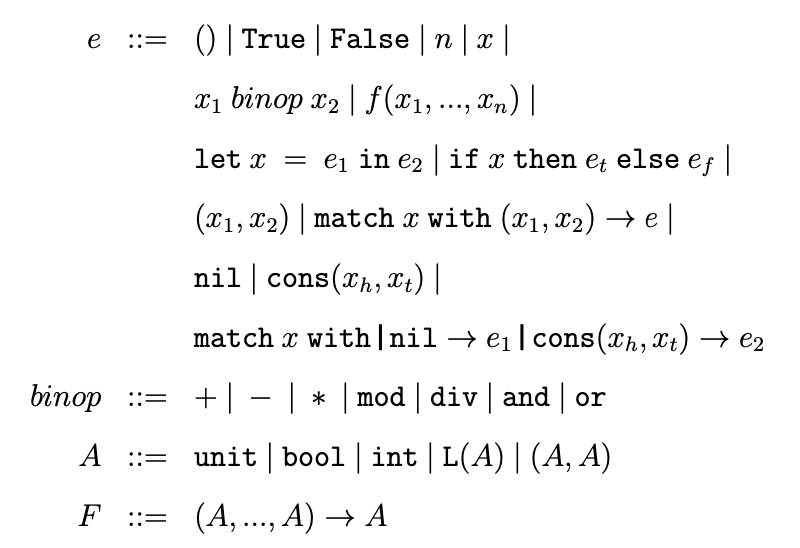
\includegraphics[scale=0.8]{image2.png}
    \caption{RAMLの文法}
    \label{image2}
  \end{center}
\end{figure}


\begin{comment}
\begin{eqnarray*}
  e &::=& ()\ {\tt |\ True\ |\ False}\ |\ n\ |\ x\ |\\
  && x_1\ binop\ x_2\ |\ f(x_1,...,x_n)\ |\\
  && {\tt let}\ x\ =\ e_1\ {\tt in}\ e_2\ |\ {\tt if}\ x\ {\tt then}\ e_t\ {\tt else}\ e_f\ |\\
  && (x_1,x_2)\ |\ {\tt match}\ x\ {\tt with}\ (x_1,x_2) \rightarrow e\ |\\
  && {\tt nil\ |\ cons}(x_h,x_t)\ | \\
  && {\tt match}\ x\ {\tt with} \mbox{\textbf |} {\tt nil} \rightarrow e_1 \mbox{\textbf |}{\tt cons}(x_h,x_t) \rightarrow e_2 \\
  binop &::=& {\tt +\ |\ -\ |\ *\ |\ mod\ |\ div\ |\ and\ |\ or} \\
  A&::=& {\tt unit\ |\ bool\ |\ int\ |\ L}(A)\ |\ (A,A) \\
  F&::=& (A,...,A) \rightarrow A
\end{eqnarray*}
\end{comment} 

図\ref{image2} にRAMLの文法を示す.$e$はRAMLプログラム上の式を表していて,
Unit値(),Boolean値{\tt True,False},整数値$n$,変数$x$,変数$x_1$と$x_2$の演算,
関数適用,let式を用いた局所関数を伴う式,ifによる条件分岐式,変数$x_1$と$x_2$のペア,
ペアに対するmatch式,空リスト{\tt nil,リストの結合を表すcons}$(x_h,x_t)$,リストに対するmatch式がある.
演算子$binop$には,整数値に対する演算である{\tt +,-,*,mod,div},
Boolean値に対する演算である{\tt and,or}がある.
$A$と$F$は,RAMLプログラム上でのsimple typeを表している.
$A$はデータ型で,Unit型の{\tt unit},Boolean型の{\tt bool},整数型の{\tt int},simple typeの値のリスト,
simple typeの値のペアがある.
$F$は関数型で,simple typeの値を受け取ってsimple typeの値を返す関数型を表している.
また,RAML上のwell-typedな式を,このsimple typeが割り当てられた式と定義している.

RAMLプログラムは,関数宣言のリストとmain式からなる.関数宣言は,関数の型宣言または関数の定義である.
それぞれの関数定義に対して型宣言を行うことができるが,プログラム内で型宣言が行われていない関数については,
プログラム実行時に型推論が行われる.main式はリソース消費量の分析の対象となる式で,プログラムの最後に記述する.


RAMLのリソース消費量の分析は,入力されたプログラムの,
big-step operational semanticsによる各評価ステップに対して一定のコストを割り当てるメトリックによって\cite{raml},
リソース消費量の計算を行う.
メトリックは以下の4つが存在する.
\begin{itemize}
  \item heapメトリックは,実行時に割り当てられたヒープセルの数を計算する.
  \item stepsメトリックは,実行時の評価ステップ数を計算する.
  \item tickメトリックは,ユーザーが定義したリソース消費であるtick値を計算する.
  ユーザーは関数の定義中に{\tt Raml.tick(1.0)}のような関数(tick関数)を呼び出すことができる.
  tick関数は呼び出される度に,引数のfloat値に等しいリソース消費(tick値)が発生する.
  \item flipsメトリックは,フリップ関数によるフリップ数を計算する.
  本論文では扱わないため,詳細な説明は省略する.
\end{itemize}

ユーザーは分析を行う際にメトリックを指定することで,
自分の注目するリソースの消費量を分析の出力として得ることができる.

RAMLプログラムの例として,リストに対するクイックソートを行うプログラムであるquicksortの
コードをCode \ref{quickraml}に示す.

\begin{lstlisting} [language=caml, caption=quicksort.raml, label=quickraml]
let rec append l1 l2 =
  match l1 with
    | [] -> l2
    | x::xs -> x::(append xs l2)

let rec partition f l =
  match l with
    | [] -> ([],[])
    | x::xs ->
      let (cs,bs) = partition f xs in
      Raml.tick(1.0);
      if f x then (cs,x::bs) else (x::cs,bs)

let rec quicksort gt = function
  | [] -> []
  | x::xs ->
      let ys, zs = partition (gt x) xs in
      append (quicksort gt ys) (x :: (quicksort gt zs))

let _ = quicksort (fun a b -> a <= b)  [9;8;7;6;5;4;3;2;1]
\end{lstlisting}

20行目の{\tt let \_ =} ...の部分はmain式を表していて,リソース消費量の分析の対象となる.
このプログラムは,{\tt append,partition,quicksort}の3つの関数を定義し,
main式は{\tt quicksort}の関数適用が記述されている.

1-4行目の{\tt append}関数は,2つのリスト{\tt l1,l2}を引数として受け取り,
それらを結合したリストを返す関数である.
6-12行目の{\tt partition関数は,リストlと,lの要素の型の値を受け取ってbool型の値を返す関数fを引数として受け取り,
lの要素をf}に関数適用したときの返り値によって2つのリストに分割する関数である.
11行目にtick関数である{\tt Raml.tick(1.0)があり,結果としてl}の要素の数だけ1.0のtick値が発生する.
14-18行目の{\tt quicksort関数は,リストlと,l}の要素の型の値を2つ受け取って{\tt bool型の値を返す関数gtを引数として受け取り,
lに対してクイックソートを実行する関数である.quicksortの定義中にappendとpartition}が用いられている.

RAMLのプログラムの実行において,主要な操作としてevaluationとanalysisの2つがある.

evaluationは,プログラムの評価を行い,main式の評価結果の返り値を出力する.
また,先述した4つのメトリックによるリソース消費量を計算し出力する.
evaluationは,{\tt ./main eval [prog.raml]というコマンドによって実行される.
ここでprog.raml}は入力として用いるプログラムファイルである.

quicksort.ramlを入力としてevaluationを実行した結果を以下に示す.

\begin{lstlisting} [basicstyle={\ttfamily\color{base}\scriptsize}]
$ ./main eval examples/quicksort.raml

Resource Aware ML, Version 1.5.0, June 2020

Typechecking expression ...
  Typecheck successful.
  Stack-based typecheck successful.

Evaluating expression ...

  Return value:
    [ 1; 2; 3; 4; 5; 6; 7; 8; 9 ]

  Evaluation steps: 1624.00
  Ticks:            36.00
  Heap space:       547.00
  Flips:            0.00

\end{lstlisting}

11-12行目に,main式の評価の返り値として,リスト{\tt [9;8;7;6;5;4;3;2;1]}が正しくソートされた値が出力されている.
また,14-17行目に,上からsteps,ticks,heap,flipsと,
それぞれのメトリックによって計算されたリソース消費量の値が出力されている.

analysisは,指定されたメトリックに則ってプログラムのリソース消費量の範囲の解析を実行する.
解析の結果として,リソース消費量の範囲が,入力されたプログラムに依存する変数の多項式として出力される.
出力される範囲は,リソース消費量の上限,下限,または上限と下限が一致した定数リソース境界から選ぶことができる.
analysisは,{\tt ./main analyze [mode] <metric> [<d1>] <d2> [-print (all | none | consume | level <lev>)] [-m] [prog.raml]} \\ {\tt [func\_name]}というコマンドで実行される.
ここで,{\tt <>は指定必須のオプションで,[]は任意のオプションである.
modeは出力される境界のタイプをupper,lower,constantから選ぶ.指定しない場合はupperとなる.
metricは分析に用いるメトリックをheap,steps,ticks,flipsから選ぶ.
d1およびd2は,リソース消費量の境界の次数を指定する.分析は次数がd1,d1+1,...,d2の範囲で行われ,
出力される多項式もその範囲の次数となる.d1を指定しない場合,d1=d2として扱われる.
-printはプログラムにおいて実行された関数の型を出力する.-printにもいくつかのオプションがあり,
-print allは実行されたすべての関数の型を出力する.-print noneは型の出力をしない.
-print level <lev>は式を構文木として見た際に深さが<lev>以下の関数の型を出力する.
-mは,指定するとモジュールモードとなり,main式の代わりにトップレベルで定義された関数の型をすべて出力する.
prog.ramlは入力として用いるプログラムファイルである.
func\_name}はモジュールモードでのみ指定することができるオプションで,指定した名前の関数についてのみ型を出力する.

quicksort.ramlを入力として,{\tt mode=upper,metric=steps,d1=1,d2=4,}
{\tt -print level 1}とオプションを設定してanalysisを実行した結果を以下に示す.

\begin{lstlisting}[basicstyle={\ttfamily\color{base}\scriptsize}]
$ ./main analyze steps 1 4 -print level 1 examples/quicksort.raml

Resource Aware ML, Version 1.5.0, June 2020

Typechecking expression ...
  Typecheck successful.
  Stack-based typecheck successful.

Analyzing expression ...

  Trying degree: 1, 2

  Function types:

== quicksort :

  [int -> int -> bool; int list] -> int list

  Non-zero annotations of the argument:
        35  <--  (*, [::(*); ::(*)])
        36  <--  (*, [::(*)])
         3  <--  (*, [])

  Non-zero annotations of result:

  Simplified bound:
     3 + 18.5*M + 17.5*M^2
   where
     M is the number of ::-nodes of the 2nd component of the argument

====

  Derived upper bound: 1624.00

  Mode:          upper
  Metric:        steps
  Degree:        2
  Run time:      0.14 seconds
  #Constraints:  638
\end{lstlisting}

11行目にTrying degree: 1,2とあるが,{\tt d1およびd2}で指定された次数1,2,3,4の低い値から順に分析を行い,
次数が2のときに分析が成功したことを示している.指定された次数において分析が成功しない場合,その旨がエラーメッセージで表示される.
15-29行目には,main式で用いられた関数{\tt quicksort}の分析の結果が示されている.
17行目に{\tt quicksortの型が示されている.[]中の型が引数の型で,複数ある場合は;}で区切られている.
19-22行目に,引数のポテンシャル注釈が引数のデータ構造ごとに示されている.
このポテンシャル注釈に関する情報を多項式に変換したものが,26-29行目に示されている.
そして,33行目にmain式の上界の値が出力され,35-39行目に分析のオプションや計算時間,計算量が出力されている.

なお,先述したようにRAMLの文法はOCamlのものを採用しているが,RAMLにおいてサポートされていないOCamlの機能がある.
以下にその例を示す.
\begin{itemize}
  \item オブジェクト指向言語としての特徴
  \item モジュール
  \item 複雑な帰納的データ型
  \item 文字列や文字
\end{itemize}


\section{RAMLでのMichelsonプログラムの実装} \label{sec-program}
本章では,RAMLを用いて,Michelsonプログラムの挙動を模倣するプログラムを実装する手法について述べる.
具体的には,Michelsonにおいて実装されている文法や命令を模倣するライブラリをRAMLにおいて設計する,
また,設計したライブラリについて,各命令において発生するガス消費量を表すtick関数を定義する.
このライブラリを用いて,Michelsonプログラムの挙動を模倣するRAMLプログラムを実装する.
第3.1節では文法について,第3.2節では命令について,第3.3節ではライブラリを用いたプログラムについて,
第3.4節ではtickメトリックを用いたガス消費量の見積もりについて述べる.
なお,実装したライブラリは本研究のGitHubレポジトリ\footnote{https://github.com/yutono326/raml}のlibrary/michleson.ramlにあるので,適宜参照されたい.

\subsection{文法} \label{subsec-pro-grammar}
Michelsonの文法は,すでに第\ref{subsec-pre-tezos}節で示した.Michelsonの文法をライブラリで設計するにあたって,
スタックの要素をOCamlのヴァリアント型を用いて表す.Code\ref{variant}に実装したヴァリアント型{\tt t}を示す.

\begin{lstlisting} [language=caml, caption=スタックの要素を表すヴァリアント型, label=variant]
type t =
  Int of int | Nat of Rnat.t | Mutez of Rnat.t |
  Bool of bool | Address | Unit | MNone | MSome of t |
  LNil | LCons of t * t | Operation | Contract |
  Pair of t * t | Left of t | Right of t 
\end{lstlisting}


ヴァリアント型{\tt tのコンストラクタとして,int型のInt,nat型のNat,mutez型のMutez,bool型のBool,
address型のAddress,unit型のUnit,option型のMNone,MSone,list型のLNil,LCons,
operation型のOperation,\\contract型のContract,pair型のPair,or型のLeft,Rightがある.
Natの引数の型であるRnat.tは,RAMLに用意されている自然数を表す型で,
四則演算add,mult,minus,div\_modと,n}が0か1以上かで分岐する条件分岐関数{\tt ifz}が関数として用意されている.
{\tt Operation,Address,Contractについては,簡略化のために引数をとらない単一のコンストラクタとして扱う.
また,list}型の要素を設計するにあたって,先述したようにRAMLにおいて複雑な帰納的データ型の実装には制限があり,
ヴァリアント型{\tt tのコンストラクタとして,t list型の値を引数にとるコンストラクタを宣言することができない.
その代替として,空リストを表すLNilと,リストの要素と元のリストを引数としてリストの結合を表すLConsをコンストラクタとして宣言する.
なお,このヴァリアント型の設計上,LCons}の2つ目の引数は型{\tt tの値である,とされているが,
コントラクトを模倣するプログラムの実行において,
LCons}の2つ目の引数が{\tt LNilまたはLConsとなるように命令の関数が定義されている.

このヴァリアント型tを用いて,スタックを型t}のリストとして設計することができる.

\subsection{命令} \label{subsec-pro-instr}
Michelsonの命令は,スタックを受け取り,そのスタックの内容を書き換える操作として実装されている.
この挙動を模倣する関数を,第\ref{subsec-pro-grammar}節で設計した文法において,
スタックに相当するリストを受け取って,書き換え後のスタックを返すような{\tt (t list $\rightarrow$ t list)}型をもつ関数として定義する.


以下,実装した関数のうち,特筆すべきものについて説明する.
\begin{itemize}
  \item {\tt FAILWITHは例外Invalid\_argumentを発生させる関数として定義する.
  \item p}は1.0のtick値を発生させる関数で,Michelsonプログラムでの{\tt \{,\}}をこれに置換する.
  後述するtickメトリックによるによるガス消費量の見積もりにおいて用いる.
  \item 中置演算子{\tt |>は,引数として受け取った2つの関数f,g}を,引数のスタックに対して続けて適用する演算子である.
  Michelsonにおける命令のシーケンスに相当する役割をもつ.
  \item {\tt LOOP}はMichelsonの挙動を再現すると解析が難しくなるため,以下に示すように
  挙動を簡単なものにしている.
  \begin{lstlisting} [language=caml]
let rec loop n body s =
  Rnat.ifz n
    (fun () ->
      match s with
      | _ :: xs -> xs
      | _ -> raise Invalid_argument)
    (fun n' ->
      match s with
      | _ :: xs -> loop n' body (body xs)
      | _ -> raise Invalid_argument)
  \end{lstlisting}
  具体的には,本来の引数に加えて{\tt Rnat.t型の引数nを受け取って,
  スタックのトップの要素に関わらず,引数の命令シーケンスをn回,スタックのトップを除いた残りのスタックに適用する関数として定義する.
  定義中に用いられるRnat.ifz}は,1つ目の引数の{\tt Rnat.t型の値n}が0ならば2つ目の引数の関数を,
  {\tt n}が1以上ならば${\tt n'=n-1}$として3つ目の引数の関数を適用する条件分岐関数である.
  \item {\tt PUSHは,受け取った要素をスタックに積む命令として定義するが,
  積む要素の型の指定はなく,値のみを引数として受け取る.
  \item ADD,SUB,MUL,EDIV}は,それぞれスタックのトップと2番目の要素を取り出し,整数値の演算結果をスタックに積む関数として定義する.
  命令にもよるが,スタックのトップと2番目の要素の型として,{\tt Int同士,Nat同士,IntとNat,Mutez同士,MutezとNatといったパターンがあり,
  パターンに応じて演算結果の要素の型が決まるので,パターンマッチングによって分ける.
  また,EDIV}ではスタックの2番目の要素が0かそうでないかで条件分岐を行い,
  スタックに積む要素の型は値のペアのオプション型となる.
  \item {\tt COMPARE}はスタックのトップと2番目の要素の比較を行い,トップの要素の方が大きい場合は{\tt Int 1}を,
  2番目の要素の方が大きい場合は{\tt Int -1を,等しい場合はInt 0をスタックに積む関数として定義する.
  Int,Nat,Mutezについて比較を行うことができるが,違う型同士の比較はできない.
  \item NONE,LEFT,RIGHT,NIL}について,Michelsonにおける命令の定義では
  それぞれオプション値,ユニオン,リストの中身の型を引数で指定する必要があるが,
  本ライブラリの関数の定義では型指定はしない.
  \item{\tt MAP,SIZE,ITERはリストに対する再帰を行う命令で,
  本ライブラリにおいてはスタックの要素が命令に合致している場合に,それぞれ対応した補助関数を呼び出す関数として定義し,
  その補助関数においてリストの再帰を行う.
  \item TRANSFER\_TOKENS,CONTRACT,SOURCE,AMOUNT}といったコントラクトに関する命令は,
  本ライブラリではコントラクトに紐づけられたアドレスや通貨量などの情報を管理することができないので,
  それらの情報を簡略化したスタック操作のみを行う関数として定義する.
\end{itemize}

\subsection{ライブラリを用いたプログラム} \label{subsec-pro-pro}
Michelsonのプログラムでは,プログラムに与えられる{\tt parameterと,ブロックチェーン上に保存されているstorageの型宣言から始まり,
parameterとstorage}のペアが積まれた初期スタックに対して,一連の命令が順番に実行される.
このプログラムの挙動を模倣するRAMLのプログラムを,設計したライブラリを用いて,
初期スタックを表すリストに対して関数を順に適用するプログラムとして実装する.

Code\ref{ex1tz}に示したプログラムexample1.tzの挙動を模倣するRAMLプログラムexample1.ramlをCode\ref{ex1raml}に示す.

\begin{lstlisting} [language=caml, caption=example1.raml, label=ex1raml]
let _ =
  (pair
  (nil
  (add
  (dip1 (p |> cdr |> p)
  (car
  (dup
  (car
  (Pair (Pair (Int 3, Int 5),  Int 0) :: []))))))))
\end{lstlisting}

プログラムの設計上,Michelsonプログラムと記述の順番が逆になっていることに注意してほしい.
Michelsonプログラムでは{\tt parameterとstorage}の型宣言から始まるが,
RAMLプログラムでは初期スタックの値を宣言し,それに対して命令に相当する関数を順に適用する.
5行目の{\tt dip1の引数となる命令シーケンスは,命令と命令の間を|>で繋ぐことによって表す.
また,シーケンスの最初と最後は\{,\}に相当するp}を記述する.

このプログラムのevaluationを実行した結果を以下に示す.

\begin{lstlisting}[basicstyle={\ttfamily\color{base}\scriptsize}]
$ ./main eval library/example1.raml

Resource Aware ML, Version 1.5.0, June 2020

Typechecking expression ...
  Typecheck successful.
  Stack-based typecheck successful.

Evaluating expression ...

  Return value:
    [ Pair ( (), LNil (), Int 8 )
                                                ]

  Evaluation steps: 249.00
  Ticks:            34.00
  Heap space:       143.00
  Flips:            0.00
\end{lstlisting}

11-13行目に,操作のリストと,{\tt parameter}として受け取った整数値の和のペアが入ったスタックが返り値として示されている.


\subsection{tickメトリックによるガス消費量の見積もり} \label{subsec-pro-gas}
スマートコントラクトのガス消費量を見積もりを行うにあたって,コントラクトを実際に実行してそのガス消費量を調べる必要がある.
コントラクトの実行環境として,Tezos開発コミュニティから提供されている仮想環境\footnote{https://gitlab.com/dailambda/docker-tezos-hands-on}を用いる.
この環境を利用する利点として,単体のコンピュータで完結していて外部のネットワークを必要としていない点,環境をいつでもリセットできる点が挙げられる.

第\ref{subsec-pre-gas}節でも述べたように,
コントラクトの実行において発生するガスの消費量は8つのコストに分けられていて,それぞれ計算方法が異なる.
ゆえに,コントラクトの実行コスト全体を見積もることは難しいと判断し,
8つのコストのうちの一つであるinterpreter costの見積もりを行うことにした.
interpreter costを選んだ理由として,命令毎にコストが設定されているので,後述する方法による見積もりがしやすいことが挙げられる.

コントラクトのinterpreter costを調べるにあたって,{\tt run script <src> on storage <storage> and input <input> --trace-stack [--gas <gas>]というコマンドを実行し,ガス消費の推移を調べるという方法を用いる.
これは,プログラムファイル\ <src>\ のスクリプトを,parameterを\ <input>,storageを\ <storage>\ とした上で実行するコマンドで,
--trace-stack}というオプションをつけることで1ステップ毎のスタックの状態,ガスの残量(使用許容量-消費量)が出力される.
{\tt --gas <gas>\ }はスクリプト開始時のガスの使用許容量を指定できるオプションである.

Code\ref{ex1tz}に示したプログラムexample1.tzについてrun scriptを実行した結果を以下に示す.

\begin{lstlisting}[basicstyle={\ttfamily\color{base}\scriptsize}]
$ ./tezos-client run script contracts/pairadd.tz on storage 0 and input 'Pair 3 5' --trace-stack --gas 100000
storage
  8
emitted operations
  
trace
  - location: 8 (remaining gas: 99655 units remaining)
    [ (Pair (Pair 3 5) 0)  	 ]
  - location: 9 (remaining gas: 99652 units remaining)
    [ (Pair 3 5)  	@parameter ]
  - location: 10 (remaining gas: 99649 units remaining)
    [ (Pair 3 5)  	@parameter
      (Pair 3 5)  	@parameter ]
  - location: 11 (remaining gas: 99646 units remaining)
    [ 3  	
      (Pair 3 5)  	@parameter ]
  - location: 14 (remaining gas: 99640 units remaining)
    [ 5  	 ]
  - location: 13 (remaining gas: 99639 units remaining)
    [ 5  	 ]
  - location: 12 (remaining gas: 99639 units remaining)
    [ 3  	
      5  	 ]
  - location: 15 (remaining gas: 99626 units remaining)
    [ 8  	 ]
  - location: 16 (remaining gas: 99620 units remaining)
    [ {}  	
      8  	 ]
  - location: 18 (remaining gas: 99612 units remaining)
    [ (Pair {} 8)  	 ]
  - location: -1 (remaining gas: 99611 units remaining)
    [ (Pair {} 8)  	 ]
\end{lstlisting}

6行目の{\tt trace}以降の出力で,1ステップ毎のスタックの状況,ガス残量が示されている.
開始時のガス許容量を{\tt 100000\ units}と指定していてるが,
最初の出力時点でいくらか減っていることから,reading cost,deserialization cost,parsing cost,type comparison costが消費された時点のガス残量が示されていると考えられる.
このガス残量から,最後の出力時点でのガス残量を引いた値がinterpreter costであると考えられる.
{\tt trace以降を見てみると,location}はプログラムの実行の進行度合いを示す値で,例えば7-10行目を見てみると,
{\tt locationが8から9になり,最初の命令であるCARが実行されてスタックが書き換えられ,ガスが3\ units消費されていることがわかる.
ここからCAR命令のinterpreter costが3\ units}であると推測できる.
また,17-23行目では{\tt DIP \{CDR\} が実行されているが,
命令のシーケンスなどにおいて\{,\}を読み込むとガスが1\ units}消費されていることがわかる.
これがinterpreter costに含まれるかどうかは定かではないが,この消費量も含めて見積もることとする.
以上の例に倣って,様々なMichelsonプログラムについてrun scriptコマンドを実行し,各命令のinterpreter costを調べた.

見積もりの方法として,tickメトリックを用いた解析を用いる.
第\ref{subsec-pro-instr}節で実装した各命令について,その命令のinterpreter costに相当する値のtick関数を呼び出すよう定義し,
ライブラリを用いて実装したプログラムをtickメトリックを用いて解析し,解析の結果として出力されるtick値の上界をinterpreter costの見積もり結果と見なす.

以下,tick関数によって正確にinterpreter costを見積もることのできない命令について述べる.
\begin{itemize}
  \item {\tt ADD,SUB,MUL,EDIV}の整数値の演算の命令におけるinterpreter costは,スタックの要素の整数値の絶対値に依存していて
  \footnote{2つの整数値の絶対値のうち大きい方を$n$とすると,$\log_2 n$に比例する.},
  それをtick関数で表すことはできなかった.ライブラリの命令においては,
  スタックの要素にに関わらず一定のtick値を発生するように定義されている.
  \item {\tt CONTRACT}命令のinterpreter costは,例外的に{\tt 10000\ units}以上となっており,
  さらに対象となるアドレスによって増減するため,設計したライブラリにおいて見積もるには情報が不十分であった.
  ライブラリの命令においては,12000.0のtick値を発生するように定義されている.
\end{itemize}

\section{解析例と考察}
以下の5つのMichelsonプログラムについて,挙動を模倣するRAMLプログラムを,
第\ref{sec-program}章で設計したライブラリを用いて実装し,
tickメトリックによる解析を行い,interpreter costの見積もりを行った.
\\
\begin{description}
  \item [example1.tz] Code\ref{ex1tz}で示したプログラム.
  \item [example2.tz] {\tt parameter}として受け取った整数値を0になるまで1ずつ減算して,ストレージに書き込む.
  \item [example3.tz] {\tt parameter}として受け取った整数値が0より大きいなら1,0以下なら-1をストレージに書き込む.
  \item [example4.tz] {\tt parameter}として受け取った整数値のリストの,要素の和をストレージに書き込む.
  \item [example5.tz] {\tt source}と呼ばれる取引が始まった実行の起点のアカウントへ受け取った通貨を送金し返す.\\
\end{description}

Michelsonプログラムexample2.tz,example3.tz,example4.tz,exmaple5.tz,
およびそれぞれを模倣するRAMLプログラムexample2.raml,example3.raml,example4.raml,exmaple5.ramlのコードを付録に付したので,
適宜参照されたい.

解析の結果を,表\ref{table1}に示す.interpreter costはrun scriptコマンドにおいて示されたinterpreter costで,
derived upper boundはRAMLプログラムの解析の結果として得られた上界である.

\begin{table}[htb]
  \begin{center}
    \caption{interpreter costの解析結果}
    \begin{tabular}{|c|c|c|} \hline
      プログラム & interpreter cost & derived upper bound \\ \hline \hline
      example1.tz & 43 & 37.00 \\ \hline
      example2.tz & 282 & 225.00 \\ \hline
      example3.tz & 28 & 28.00 \\ \hline
      example4.tz & 80 & failed \\ \hline
      example5.tz & 12079 & 12079.00 \\ \hline
    \end{tabular}
    \label{table1}
  \end{center}
\end{table}

example1.ramlとexample2.ramlの解析結果については,interpreter costとderived upper boundに多少の開きがあるが,
これは,{\tt ADD}命令のinterpreter costがスタックの要素の整数値の絶対値に依存している点が
RAMLの解析において考慮されてないことに起因していて,それを除けば正しく見積もることができたと言える.
example4.ramlについては解析自体が正しく行われなかった.
これは,リストに対する再帰を行う命令である{\tt ITER}命令がプログラムに含まれていたことが原因であると考えられる.
example5.ramlは{\tt CONTRACT命令を含んだプログラムで,正確な解析はできないと先述したが,
このプログラムにおけるCONTRACT}命令のinterpreter costが12000unitsであったため,解析結果として正しい上界が得られた.

example4.ramlの解析に関して,以下に示すような{\tt iter\_list}の関数適用のみを行うプログラムついての解析は行うことができる.
\begin{lstlisting} [language=caml]
let _ =
  iter_list (p |> add |> p) (LCons (Int 1, LCons (Int 2, LCons (Int 3, LCons (Int 4, LNil)))) :: Int 0 :: [])
\end{lstlisting}
このプログラムの解析結果として得られる上界が32.00であることから,
以下のようにexample4.ramlの{\tt iter\_list}の部分を置き換えることで,プログラムの解析を行うことができる.
\begin{lstlisting} [language=caml]
let f s = Raml.tick(32.0); Int 10 :: []

let _ =
  (pair
  (nil
  (f
  (dip1 (p |> push (Int 0) |> p)
  (car
  (Pair (LCons (Int 1, LCons (Int 2, LCons (Int 3, LCons (Int 4, LNil)))), Int 0) :: []))))))
\end{lstlisting}

しかし,example4.ramlのような{\tt iter\_list}を含む関数を連続適用するプログラムについて解析が正しく行われなかった点については,
詳細な原因はわからなかった.

\section{関連研究} \label{sec-relate}
スマートコントラクトを対象とした静的な解析は,本研究で示したガス消費量の解析の他にも様々な目的で研究されている.
その中でも,ブロックチェーン技術が幅広い用途に利用されるにつれ,スマートコントラクトが扱うデータの重要性も高まっており,
大量の通貨をスマートコントラクト上で取り扱うため,プログラムを静的かつ形式的に検証する手法への需要が高まっている.

西田らは,Tezosのスマートコントラクト言語Michelsonの静的型検証ツールHelmholtzを開発した\cite{helmholtz}\cite{hurui}.
Helmholtzの開発にあたって,Mihchelsonのための篩型システムを単純型システムの拡張として実装している.
この篩型システムは,スタックの型に対して条件を付けるシステムである.
Helmholtzは,篩型の形式で表現され,ユーザーの定義した注釈が付けられたMichelsonプログラムを受け取る.
次に,篩型システムに基づく仕様の注釈の入ったプログラムに対する型検査が行われ,
型検査中に生成された検証条件はSMTソルバであるZ3\cite{z3}によって検証される.
Helmholtzの検証において,コードが正しく型付けされているプログラムは仕様を満たすことが保証される.

\section{結論}\label{sec-conclusion}
\subsection{結論} \label{subsec-conclusion-conclusion}
本研究では,RAMLを用いて,Tezosのスマートコントラクトのガス消費量を静的に解析する手法を提案した.
Tezosのスマートコントラクトはスタックベースのプログラミング言語であるMichelsonで記述されていて,
その挙動をRAMLで再現するために,スタックの要素を独自のヴァリアント型の値として定義し,
MIchelsonの各命令を,スタックを表すリストを受け取ってその内容を変更して返す関数として定義し,
Michelsonプログラムを初期スタックを表すリストに対して命令を順に関数適用するRAMLプログラムとして実装した.
ガス消費量の見積もりについては,コントラクトの実行に伴うガス消費量のうちinterpreter costを見積もることを目的とし,
RAMLのtickメトリックを用いてプログラムの解析を行う手法を示した.

いくつかのコントラクトについて解析を行い,interpreter costを見積もった結果,
基本的なスタック操作や条件分岐の命令のみで構成されているコントラクトについては解析が成功し,
interpreter costを正しく見積もることができた.
一方で,リストや集合に対する再帰を行う命令を含むコントラクトでは解析が行えなかった.
また,ガス消費量がスタック中の値に依存するような命令を含むコントラクトについては,
正しくinterpreter costの見積もりを行うことは難しかった.

\subsection{今後の課題} \label{subsec-conclusion-work}
本研究では,Michelsonに実装されている命令のうち主要な命令についてRAMLライブラリで扱えるように実装した一方で,
setやmap,関数などの型は実装しておらず,それらに関連する命令も実装されていない.
本ライブラリにおいてより多くのプログラムを扱えるように,実装を進めていく予定である.
また,リストの再帰を行う命令を含むコントラクトの解析が正しく行えなかった点について,リスト型の実装方法に問題があった可能性がある.
これを正しく解析できるようにするために,実装体系を見直すことも検討している.

また,コントラクトの実行に伴うガス消費量のうち,interpreter costを見積もる手法を示したが,
interpreter costはコントラクトの実行コスト全体のごく一部に過ぎない.
コントラクトの実行コスト全体の見積もりを行うために,その他のコストの計算方法について研究し,
解析を行うことも今後の課題である.


\acknowledgments
本報告書の執筆にあたり,多くの方々に支援いただきました.
本研究に取り組むにあたって,研究テーマを提示して頂き,終始適切な助言を賜り,丁寧に指導して下さった末永幸平准教授に心より感謝いたします.
また,TezosやMichelsonの体系や様々な知識について解説して頂いた古瀬淳氏と,基本的なMichelsonコードを提供して頂いた斉藤大聖氏に感謝いたします.
そして,本報告書の執筆にあたって,添削や助言を頂いた五十嵐淳教授,和賀正樹助教をはじめ,多くの助言を頂いた五十嵐・末永研究室の皆様に深く感謝いたします.

\nocite{*}
\bibliographystyle{kuisunsrt}
\bibliography{main}

\appendix
第4章において用いたMichelsonプログラムと,それを模倣するRAMLプログラムのコードを以下に示す.

\begin{lstlisting} [language=michelson, caption=example2.tz, label=ex2tz]
parameter int;
storage int;
code {  CAR ;
        DUP ;
        GT ;
        LOOP { PUSH int -1 ; ADD ; DUP ; GT } ;
        NIL operation ;
        PAIR  }
\end{lstlisting}

\begin{lstlisting} [language=michelson, caption=example3.tz, label=ex3tz]
parameter int;
storage int;
code {  CAR ;
        GT ;
        IF {PUSH int 1} {PUSH int -1} ;
        NIL operation ;
        PAIR  }
\end{lstlisting}

\begin{lstlisting} [language=michelson, caption=example4.tz, label=ex4tz]
parameter (list int);
storage int;
code {  CAR ;
        DIP { PUSH int 0 } ;
        ITER { ADD } ;
        NIL operation ;
        PAIR  }
\end{lstlisting}

\begin{lstlisting} [language=michelson, caption=example5.tz, label=ex5tz]
parameter unit;
storage unit;
code {  CDR ;
        NIL operation ;
        AMOUNT ;
        PUSH mutez 0 ;
        COMPARE ;
        EQ ;
        IF
          {}
          { SOURCE ; CONTRACT unit ; { IF_NONE FAILWITH {} } ; AMOUNT ; UNIT ; TRANSFER_TOKENS ; CONS } ;
        PAIR  }
\end{lstlisting}

\begin{lstlisting} [language=caml, caption=example2.raml, label=ex2raml]
let _ =
  (pair
  (nil
  (loop (Rnat.of_int 10) (p |> push (Int (-1)) |> add |> dup |> gt |> p)
  (gt
  (dup
  (car
  (Pair (Int 10, Int 0) :: [])))))))
\end{lstlisting}

\begin{lstlisting} [language=caml, caption=example3.raml, label=ex3raml]
let _ =
  (pair
  (nil
  (if_ (p |> push (Int 1) |> p) (p |> push (Int (-1)) |> p)
  (gt
  (car
  (Pair (Int 5, Int 0) :: []))))))
\end{lstlisting}

\begin{lstlisting} [language=caml, caption=example4.raml, label=ex4raml]
let _ =
  (pair
  (nil
  (iter_list (p |> add |> p)
  (dip1 (p |> push (Int 0) |> p)
  (car
  (Pair (LCons (Int 1, LCons (Int 2, LCons (Int 3, LCons (Int 4, LNil)))), Int 0) :: []))))))
\end{lstlisting}

\begin{lstlisting} [language=caml, caption=example5.raml, label=ex5raml]
let _ =
  (pair
  (if_ (p |> p) (p |> source |> contract |> if_none failwith (p |> p) |> amount |> unit |> transfer_tokens |> cons |> p)
  (eq
  (compare
  (push (Mutez Rnat.zero)
  (amount
  (nil
  (cdr
  (Pair (Unit, Unit) :: [])))))))))
\end{lstlisting}

\end{document}